\htwo{Containertechnologie und Docker}
\label{sec:ContainerAndDocker}
\sectionauthor{Richard Panzer}

Docker ist eine Software, welche die Inbetriebnahme von Linux Containern ermöglicht. Da Docker eine Open-Source Plattform ist, kann sie von der Community ständig weiterentwickelt werden. Das Unternehmen Docker Inc. unterstützt und verbessert die kostenlose Arbeit der Community und bietet professionellen Support. Sollte das Unternehmen jedoch auf eine Verbesserung gestoßen sein, so teilt es diese auch mit allen Entwicklerinnen und Entwicklern der Open-Source Community. Außerdem fokussiert sich die Docker Inc. auf die Betreuung von Unternehmenskundinnen und Unternehmenskunden, um zuverlässigere Anwendungen zu entwickeln. \cite{Docker}

 \hthree{Linuxcontainer}

Da die moderne Computer- und Entwicklungswelt immer komplexer und anspruchsvoller wird, bietet die Containertechnologie mithilfe von Linux-Containern die Möglichkeit unterschiedliche Anwendungen samt ihren gesamten Daten quasi zu paketieren und vom Rest des Systems zu isolieren.  So blieben die einzelnen Programme und Anwendungen uneingeschränkt funktionsfähig und können in einzelnen Umgebungen verschoben werden, wie die Entwicklung oder die Produktion. \cite{Container}

Der entscheidende Grund sich für die Entwicklung mit Containertechnologie zu entscheiden, liegt darin, dass man so Konflikte zwischen den Entwicklern und Operationsteam trennen kann, da die Zuständigkeiten dieser zwei Teams auch völlig unterschiedlich sind. So arbeiten Systemapps und Systeminfrastruktur voneinander getrennt und in separaten Containern. Der wohl wichtigste Vorteil Linux-Container als gewünscht Technologie zu wählen, liegt daran, dass diese Technologie open Source basiert ist und so Änderungen und Erneuerung sofort und kostenlos für alle zur Verfügung gestellt werden. \cite{Container}

 \hthree{Containersicherheit}

Unter dem Überbegriff "Containersicherheit", wird der Schutz eines Container in einem System verstanden und hierbei die Abwicklung eines Prozesses, eines Services, oder aber auch die gesamte Systeminfrastruktur des Services. \cite{ContainerSecurity}

\begin{figure}[H]
    \centering
    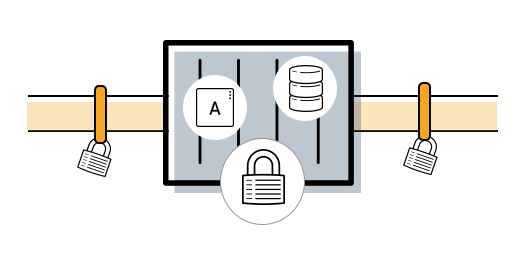
\includegraphics[width=\textwidth]{media/DockerAndContainering/Containersicherheit.png}
    \caption{Containersicherheit \cite{ContainerSecurity}}
\end{figure}

\hfour{Imagesicherheit}

Container oder besser gesagt Services, welche in Containern laufen gelassen werden, werden über sogenannte "Images" bereitgestellt. Dies bietet die Möglichkeit, direkt über ein schädliches "Image" Schadsoftware oder Sicherheitslücken direkt beim Initialisieren des Systems mitzuinstallieren, oder zu öffnen. Wichtig ist daher, dass das "Basisimage", also der Ausgangspunkt für weitere "Images" und Services sicher und geschützt ist. \cite{ContainerSecurity}

Es ist daher wichtig, dass die Entwickler*innen nur "Images" verwenden, welche vertrauenswürdig und sicher sind. Eine 100\% Sicherheit kann jedoch nie gewährleistet sein, da durch das Verändern der Konfiguration oder dem Hinzufügen von neuen Anwendungen wieder Sicherheitslücken entstehen können. \cite{ContainerSecurity}

Ein sicherer Ort für das Auswählen und Verwenden von "Images" ist der "Docker Hub", da im Menü auf der rechten Seite ausgewählt werden kann, ob der Ersteller des "Images" ein verifizierter Ersteller sein muss. \cite{ContainerSecurity}

\begin{figure}[H]
    \centering
    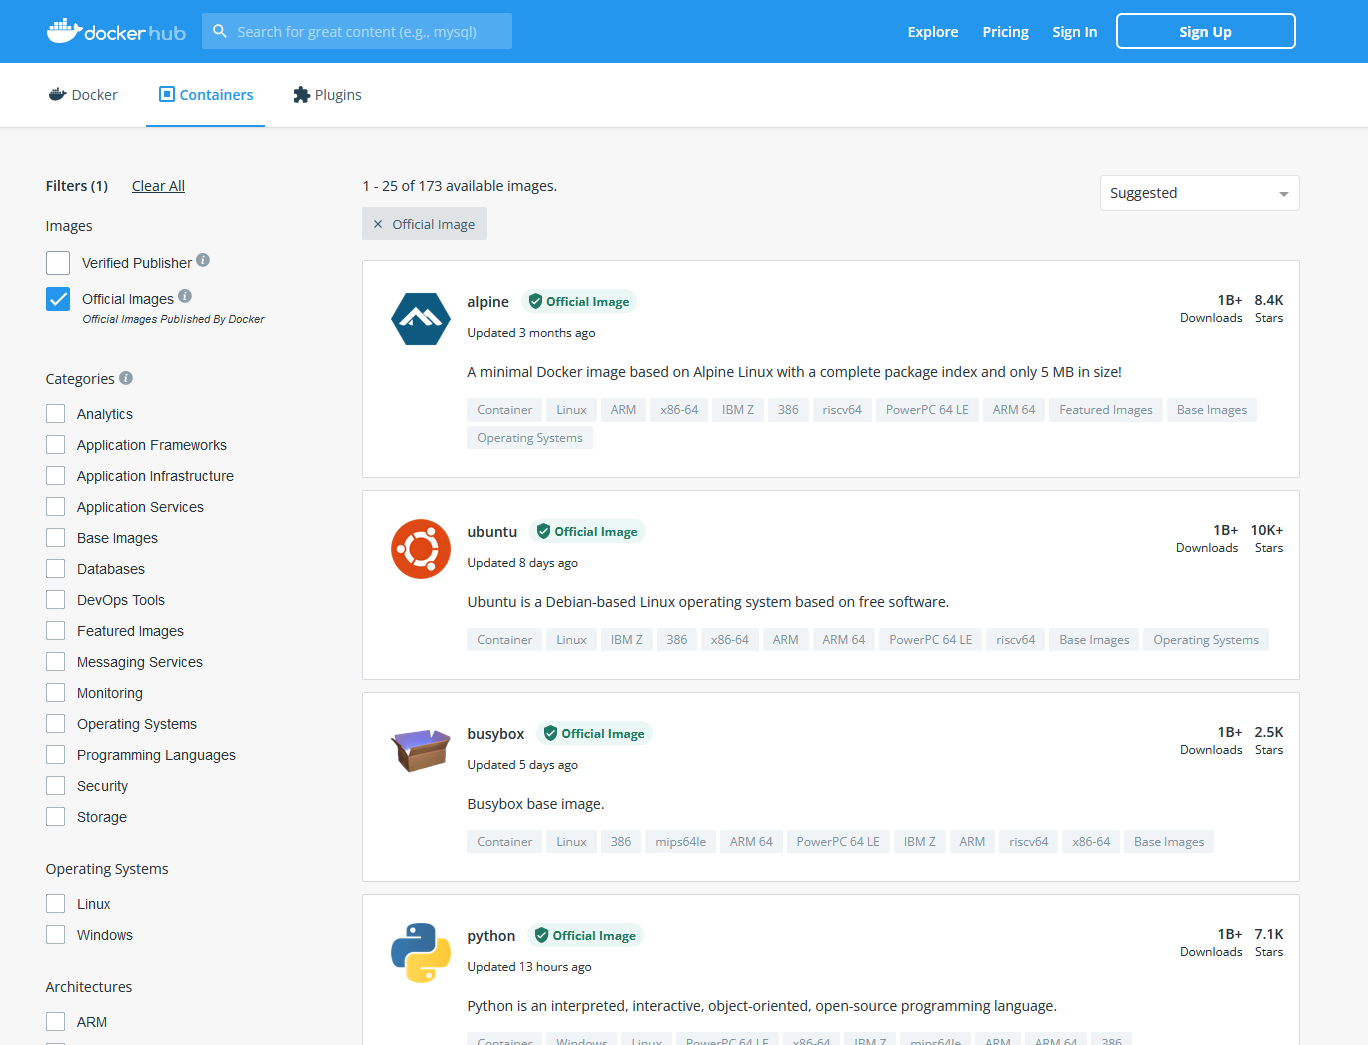
\includegraphics[width=\textwidth]{media/DockerAndContainering/DockerHub.png}
    \caption{"Docker Hub" \cite{DockerHub}}
\end{figure}

Zusammengefasst kann gesagt werden, dass sich vor der Auswahl eines "Images" die Entwickler*innen folgende Fragen stellen sollten:

\begin{itemize}
    \item "Sind diese Images signiert bzw. stammen Sie aus vertrauenswürdigen Quellen?" \cite{ContainerSecurity}
    \item "Sind Runtime- und Betriebssystemschichten aktuell?" \cite{ContainerSecurity}
    \item "Wie schnell und häufig werden die Container aktualisiert?" \cite{ContainerSecurity}
    \item "Wird auf bekannte Probleme überwacht, und wann ja, wie?" \cite{ContainerSecurity}
\end{itemize}

\hfour{Zugriffsverwaltung}

Nachdem der Container nun mit dem gewünschten "Image" richtig aufgesetzt wurde, ist es nun wichtig den Zugriff auf diesen abzusichern. Egal ob der Container nun entwickelt wird (zum Beispiel ein Datenbankcontainer) oder einen Service (beispielsweise einen Service zum Herunterladen) bereitstellt. 

Der Zugriff auf den Container kann durch eine sogenannte "Private Registry" rollenbasiert geregelt werden. Über "Metadaten" kann die Kontrolle von den Daten, auf welche zugegriffen werden soll, kontrolliert werden. Bei "Metadaten" werden beispielsweise schon bekannte Sicherheitslücken weiterverfolgt, oder nach neu auftretenden gesucht. Durch "Private Registry" werden globale Richtlinien für Container und deren "Images" automatisch bereitgestellt. Dies hat den Vorteil, dass menschliches Versagen im Bereich der Richtlinien minimiert werden kann. \cite{ContainerSecurity}

Die Entwickler*innen sollten sich im Bereich der Zugriffsverwaltung Antworten zu folgende vier Fragen überlegen:

\begin{itemize}
    \item "Welche rollenbasierten Kontrollen können Sie für das Management von Container Images nutzen?" \cite{ContainerSecurity}
    \item "Stehen Tagging- oder Kennzeichnungsfunktionen zur Unterstützung der Image-Sortierung zur Verfügung? Können Sie Images separat für Entwicklung, Prüfung und Produktion als genehmigt kennzeichnen?" \cite{ContainerSecurity}
    \item "Bietet die Registry sichtbare Metadaten, mit denen Sie auf bekannte Schwachstellen überwachen können?" \cite{ContainerSecurity}
    \item "Lässt sie sich zur Zuweisung und Automatisierung von Richtlinien (z. B. Prüfung von Signaturen, Codierung von Scans etc.) einsetzen?" \cite{ContainerSecurity}
\end{itemize}

\hfour{Deployment}

Im folgenden Schritt geht es nun darum, das fertige Endservice fortlaufend auf Sicherheitslücken zu prüfen. Sollte eine Lücke entdeckt worden sein, kann diese entweder durch einen "Patch" oder einen "Rebuild" geschlossen werden. "Patches" werden eher nicht gemacht. Es werden eher anhand automatischer Prüfungen Lücken entdeckt und durch automatische Updates und einen "Rebuild" geschlossen. Außerdem bleibt das komplette Neuaufsetzen eines Containers inklusive des Services. \cite{ContainerSecurity}

Bei der Sicherheit im Deploymentbereich sollten die Entwickler*innen folgende Frage beantworten:

\begin{itemize}
    \item "Wie können Sie das Patching ausgeführter Container vermeiden und sie stattdessen per Trigger mithilfe automatischer Updates neu erstellen bzw. ersetzen?" \cite{ContainerSecurity}
\end{itemize}

\cite{ContainerSecurity}

\hfour{Infrastruktur}

Um in diesem Bereich Sicherheit zu bekommen sind die Entwickler*innen auf das Betriebssystem der Hostmaschine angewiesen. Es ist wichtig, dass das Betriebssystem eine hohe Isolierung zwischen den einzelnen Containern bietet und damit Sicherheit bringt. Jedoch kann über "Netzwerk-Namespaces" beispielsweise eine gemeinsame Nutzung von Speicher zwischen den Containern ermöglicht werden. Es sollte aber jede Anwendung auch die nötigen Sicherheitsvorkehrungen (Authentifizierung, Autorisierung, Durchsatzbeschränkungen, usw.) implementiert haben, um sich nicht rein auf die Containersicherheit oder die Infrastruktursicherheit zu verlassen. \cite{ContainerSecurity}

Die Entwickler*innen sollten sich aber im Bereich der Infrastruktursicherheit bei der Implementierung folgende Fragen stellen:

\begin{itemize}
    \item "Welche Container müssen aufeinander zugreifen können? Wie können sich Container gegenseitig ermitteln?" \cite{ContainerSecurity}
    \item "Wie sollen der Zugriff auf und das Management von gemeinsamen Ressourcen (z. B. Netzwerk und Storage) kontrolliert werden?" \cite{ContainerSecurity}
    \item "Wie werden Host-Updates verwaltet? Müssen all Ihre Container gleichzeitig aktualisiert werden?" \cite{ContainerSecurity}
    \item "Wie überwachen Sie den Container-Zustand?" \cite{ContainerSecurity}
\end{itemize}

 \hthree{LXC VS. Docker}

\hfour{Architektur}

Im Kern ähnelt sich die Systemarchitektur von LXC jener von Docker, da die wichtigsten verwendeten Funktionen des Linux-Kernel "cgroups" und "namespaces" sind. "cgroups" sind hierbei für die Aufteilung von CPU, Speicher und vielem mehr im System zuständig. "Namespaces" erlauben das Erstellen von mehreren virtuellen Instanzen des Kernels. Es kann daher gesagt werden, dass sich LXC und Docker im Bereich des Systemkernels sehr ident sind. \cite{LxcVsDocker}

Im Bereich der Engine, welche zwischen Anwendung und Kernel liegt, setzt LXC auf das Framework "liblxc". Docker implementierte jedoch ihre eigene Engine, welche den Namen "libcontainer" trug. Diese wurde jedoch im Laufe der Jahre durch mehrere dazwischenliegende Abstraktionsschichten ergänzt. \cite{LxcVsDocker}

Die gesamte Architektur von Docker ist jedoch nicht ganz so trivial. Der grobe Ablauf beim Zugriff auf Daten sieht wie folgt aus:

Zu Beginn greift der Client auf den "Docker Deamon" zu, welcher auf einem "Docker\_Host" liegt. Dieser stellt die Hauptbenutzeroberfläche zur Verfügung. Der "Docker Deamon" greift nun auf ein Image im Host zu, welches schreibgeschützt ist. Es kann jedoch Images mehrere Container geben, auf welchen dann die gewünschten Änderungen des Clients durchgeführt werden. \cite{LxcVsDocker}

\begin{figure}[H]
    \centering
    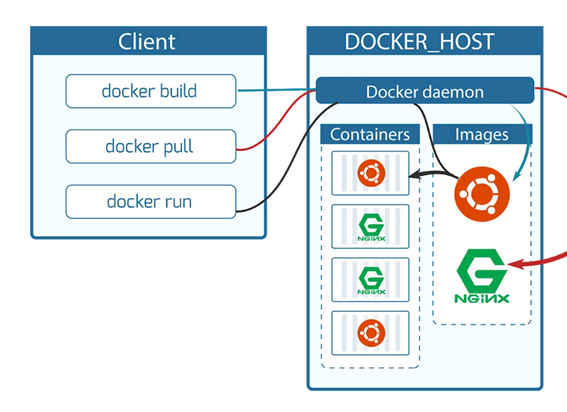
\includegraphics{media/DockerAndContainering/DockerArchitektur.png}
    \caption{Docker Architektur \cite{LxcVsDocker}}
\end{figure}

\hfour{Speicherverwaltung}

Bei LXC ist die Speicherverwaltung recht einfach gemacht worden. Sofern keine anderen Optionen gewählt wurden, legt LXC die Daten unter dem Linux Pfad: "/var\-/lib\-/lxc\-/[container-name]/rootfs" ab. Die Einbindung von Datenbanken oder eines NAS-Systems (Network Attached Storage) funktioniert ohne große Probleme, da alles über das "rootfs" des jeweiligen Containernamen abgewickelt wird. \cite{LxcVsDocker}

Bei Docker funktioniert das Ganze ein bisschen anders. Hierbei wird das Image normal in seiner Gesamtheit abgelegt. Das Image verweist jedoch auf eine Vielzahl von Speicherebenen, welche eben einem Image eindeutig zugeordnet sind. Diese Ebenen werden beim Erzeugen übereinandergestapelt. Dieser Speicherstapel des Images ist dann die Basis des sogenannten "Container-Root-Dateisystems". Für das Übereinanderstapeln und das generelle Verwalten der Speicherebenen ist der Treiber des "Docker Storage" zuständig. Außerdem verwaltet dieser Treiber auch das gemeinsame Verwenden von Speicherebenen zwischen Containern. Ein Vorteil, welcher sich einerseits aus diesem Verwaltungsmechanismus und andererseits aus der gegenseitigen Nutzbarkeit ergibt, ist auf der einen Seite das vereinfachte Erstellen, Verschieben oder Kopieren des gesamten Images und auf der anderen Seite spart die gemeinsame Nutzung Speicherplatz auf dem System. \cite{LxcVsDocker}

Sobald die User*innen einen neuen Container erzeugen, passiert Folgendes: Es wird auf das angegebene Image zugegriffen, welches jedoch schreibgeschützt ist. Deshalb bekommt jeder einzelne Container eines Images eine eigene Speicherebene in diesem Gesamtimage. So greift jeder Container nur auf seinen Speicherstand zu und man kann von einem Image auch mehrere unterschiedliche Speicherstände haben. \cite{LxcVsDocker}

\begin{figure}[H]
    \centering
    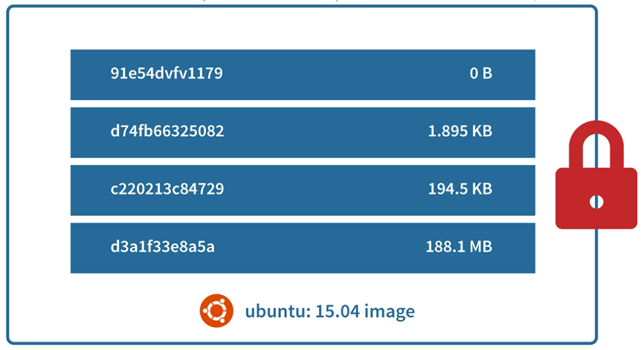
\includegraphics[width=0.9\textwidth]{media/DockerAndContainering/Speicherebenen.png}
    \caption{Speicherebenen in Docker \cite{LxcVsDocker}}
\end{figure}

Docker arbeitet beim Schreiben oder Ändern von Images oder Containern mit der sogenannten "Copy-on-Write"(CoW)-Technologie. Dies ist ein Optimierungsverfahren, welches für das Schreiben zwischen zwei Prozessen auf unixartigen Systemen eingesetzt wird. Die Grundidee dahinter ist, dass eine Kopie einer Datei erst real angelegt wird, wenn sie sich von der "Mutterdatei" unterscheidet. Für Docker bedeutet das eine Optimierung von der Nutzung des Plattenplatzes und bessere Startzeiten für die jeweiligen Container. \cite{LxcVsDocker}

 \hthree{Testumgebungen durch Containertechnologien}

Durch das Einsetzen von unterschiedlichsten Containertechnogien wie Docker, wird es Administratorinnen oder Administratoren leichter gemacht, eine simple aber vor allem effiziente Testinfrastruktur und Testumgebung schnell und unkompliziert zu implementieren. Sollte zum Beispiel eine Version eines bestimmten Services einen Fehler beinhalten, können Container aushelfen. So können die Entwickler*innen denselben Service auf zwei unterschiedlichen Versionen in zwei separierten Containern laufen lassen und individuell prüfen, ab welcher Version der Fehler auftritt. Außerdem können Container innerhalb kürzester Zeit gestartet und die Testumgebung angeworfen werden. Dies hat den großen Nutzen, dass kleine Infrastrukturänderungen, welche ab und an nötig sind, durch das Verwenden von Containertechnologie keine Probleme mehr darstellen. \cite{TestenContainer}

Größere und komplexere Testszenarien können so durch die neu erlangte Flexibilität im Testen von Software und Systemen unterschiedlichster Art einfach und für die Administratorinnen und Administratoren unkompliziert abgewickelt werden. Außerdem kann man das Testsystem, welches sich in einem Linux Container befindet, leichter transportieren als ein physisches System. \cite{TestenContainer}

 \hthree{Wie funktioniert Docker}
\label{sec:dockerexplained}

Die Docker Technologie greift auf den Linux Kernel zurück, um die gewünschten Funktionen bereit zu stellen. Hierbei wird vom Kernel auf der einen Seite auf die sogenannten Kontrollgruppen zugegriffen, welche zum Beispiel für die CPU-Zeit, den Systemspeicher, oder die Netzwerkbandbreite und deren Aufteilung auf verschiedene Prozesse zuständig sind, als auch auf die "User Namespaces". So schafft es Docker, Prozesse und Applikationen getrennt und isoliert voneinander laufen zu lassen. \cite{Kontrollgruppen} \cite{DockerGrundlagen}

Docker ist ein imagebasiertes Bereitstellungsmodel und schafft es so Anwendungen und Pakete von Services gleichzeitig in unterschiedlichen Containern dem Anwender bereitzustellen. \cite{DockerGrundlagen}

Es ermöglicht die Bereitstellung von Container mit guter Performance und individueller Kontrolle der einzelnen Services und Versionen der Services. \cite{DockerGrundlagen}
 \hthree{Vorteile von Docker}

\hfour{Modularität}

Docker Container fokussieren sich darauf, beim Ausfall oder der Aktualisierung eines Teils der Anwendung nicht das ganze System herunterzufahren, sondern nur den Teil, welcher wirklich davon betroffen ist. Weiters macht dieser microbasierte Ansatz es auch möglich, dass Prozesse von mehreren Anwendungen gleichzeitig genutzt werden können. \cite{DockerGrundlagen}

\hfour{Layer- und Image-Versionskontrolle}

Jedes Image in Docker ist in den einzelnen Bestandteilen in Layern organsiert. Jeder einzelne Layer ist einem Image fix zuzuordnen. Bei jeder Veränderung oder Abänderung, welche ein Image betrifft, wird ein neuer Layer erstellt. Dies kommt zum Beispiel bei der Eingabe der Befehle: "docker run" oder "docker copy" vor. \cite{DockerGrundlagen}

Die erstellten Layer aus alten Images werden beim Erstellen von neuen Containern wiederverwendet. Dies beschleunigt die Erstellung neuer Container gewaltig. Weiters können Änderungen, welche während des Betriebes passieren, von allen Docker Containern gleichzeitig verwendet werden, um so noch mehr Performance herauszuholen. \cite{DockerGrundlagen}

In Bezug auf die Versionskontrolle kann Folgendes gesagt werden: Durch die Containerorganisierung in Layern, welche immer ein Änderungsprotokoll enthalten, habe ich immer die gesamte Kontrolle über meine Docker Container. \cite{DockerGrundlagen}

\hfour{Rollback}

Layer bieten auch den Vorteil, Rollbacks, also das Zurückkehren auf eine ältere Version, sehr einfach und elegant umzusetzen. Sollte der Entwickler oder die Entwicklerin mit der aktuellen Version eines Images nicht zufrieden sein, so ist ein Rollback über Layer organisiert einfach zu bewerkstelligen. Der hier implementierte Standard eines Rollbacks unterstützt auch die agile Entwicklung und die kontinuierliche Integration und Bereitstellung. \cite{DockerGrundlagen}

\hfour{Schnelle Bereitstellung}

Für den Fall, dass ein Unternehmen neue Hardware benötigt, dauert es oft lange, bis diese voll funktions- und einsatzfähig ist und ist mit einem großen Aufwand verbunden. Durch Docker reduziert sich dieser Aufwand auf ein Minimum. Durch das Organisieren von Prozessen in Containern, kann ich Prozesse ganz einfach unterschiedlichen Applikationen gleichzeitig und innerhalb von wenigen Minuten bereitstellen. Weiters muss die Stammmaschine beim Hinzufügen oder Verschieben eines Containers nicht neu gebootet werden, wodurch Ausfallzeiten des Systems minimiert werden. \cite{DockerGrundlagen}

 \hthree{Docker Inc.}

Docker Inc. ist ein US-amerikanisches Unternehmen mit Hauptsitz in San Francisco im Bundesstaat Kalifornien, welches im Jahr 2013 gegründet wurde. Der Chief Executive Officer des Unternehmens ist Scott Johnston, der diese Funktion seit 2014 innehat. Das Unternehmen ist wie der Name schon sagt im Bereich der Technologie von Linux Containern tätig. Ein weiters Spezialgebiet von Docker Inc. ist das Arbeiten mit und Entwickeln von Open-Source Anwendungen, da insgesamt über 13 Millionen Menschen an Docker arbeiten und es stätig weiterentwickeln. Hauptberuflich arbeiten bei Docker Inc. zwischen 51 und 200 Beschäftigte. \cite{DockerInc} \cite{Docker}

 \hthree{Docker Desktop}

Docker Desktop ist eine Software, um Docker Container auf seinem Rechner anzulegen und zu erstellen. Sie wurde mit der ersten Betaversion am 21. Dezember 2013 veröffentlicht. Die erste Produktionsversion wurde am 16. Oktober 2014 herausgebracht. Die aktuelle Version (4.2.0) wurde am 9. November 2021 zur Verfügung gestellt. \cite{DockerWiki}
 \hthree{Docker vs Virtuelle Maschinien}

Die Technologie und der Sinn von Docker unterscheiden sich in vielen Punkten von herkömmlichen Virtuellen Maschinen. Jedoch kann man zusammenfassend und vereinfacht sagen, dass virtuelle Maschinen für die meisten Benutzer einmal erstellt und nachher nicht mehr geändert werden. Die VM muss höchstens aktualisiert, umkonfiguriert oder repariert werden. Jedoch bleibt sie immer ein sich geschlossenes System.

Oft wird davon gesprochen, dass die Linux-Containertechnologie und im speziellen Docker Virtuelle Maschinen überflüssig machen. Dieser Gedankengang ist jedoch falsch, da die beiden Technologien zwei unterschiedliche Anwendungsgebiete abdecken sich ergänzen, aber nicht ersetzen. Auf der einen Seite bieten VMs den Vorteil, dass sie Infrastrukturelastizität bieten, auf der anderen Seite hat Docker den Vorteil, dass die Software wie einzelne Bausteine zusammengesetzt ist. So schafft man es, moderne Architektur-Ansätze unveränderbar und verteilte zu implementieren. \cite{DockerVsVm}

